\documentclass[10pt]{article}
\usepackage[english]{babel}
\usepackage{../../../meta-inf/lib/naproche}
\usepackage{amssymb}
\usepackage{mathtools} % for \coloneq

\usepackage{stex-highlighting}
\providebool{emph} % "\newbool{emph}" does not work...
\setbool{emph}{false}
\colorlet{emphcolor}{violet}
\let\oldemph\emph
\renewcommand\emph[1]{\setbool{emph}{true}\ifbool{forthel}{\textcolor{emphcolor}{\itshape#1}}{\oldemph{#1}}\setbool{emph}{false}}
\renewcommand{\varemph}[1]{\ifbool{emph}{\textcolor{emphcolor}{#1}}{\textcolor{black}{#1}}}

\usepackage[right=6cm,left=3cm,bottom=3cm,marginparwidth=5cm]{geometry}

\usepackage{fancyhdr}
\renewcommand{\sectionmark}[1]{\markboth{#1}{}} 
\def\libarchive{}
\pagestyle{fancy}
\fancyhead[L]{\libarchive}
\fancyhead[C]{\nouppercase\leftmark}  % section title
\fancyhead[R]{\thepage}               % page number
\fancyfoot[C]{}                       % No page number in footer

\usepackage[nobottomtitles]{titlesec}
\titlespacing*{\section}{0pt}{30pt}{0pt}
\titlespacing*{\subsection}{0pt}{30pt}{0pt}
\titlespacing*{\subsubsection}{0pt}{30pt}{0pt}

\documentclass[12pt,oneside]{book}

\usepackage[foundations]{../../lib/tex/naproche}
\usepackage{../../lib/tex/libraries}
\usepackage{graphicx}
\usepackage{float}
\usepackage{caption}
\usepackage{footnote}

\makesavenoteenv{tabular} % Make footnotes work in tabular environments


\title{Foundations of Mathematics}
\author{Marcel Schütz}
\date{2022}

\begin{document}
  \maketitle

  \tableofcontents

  \begin{figure}[H]
    \centering
    \fbox{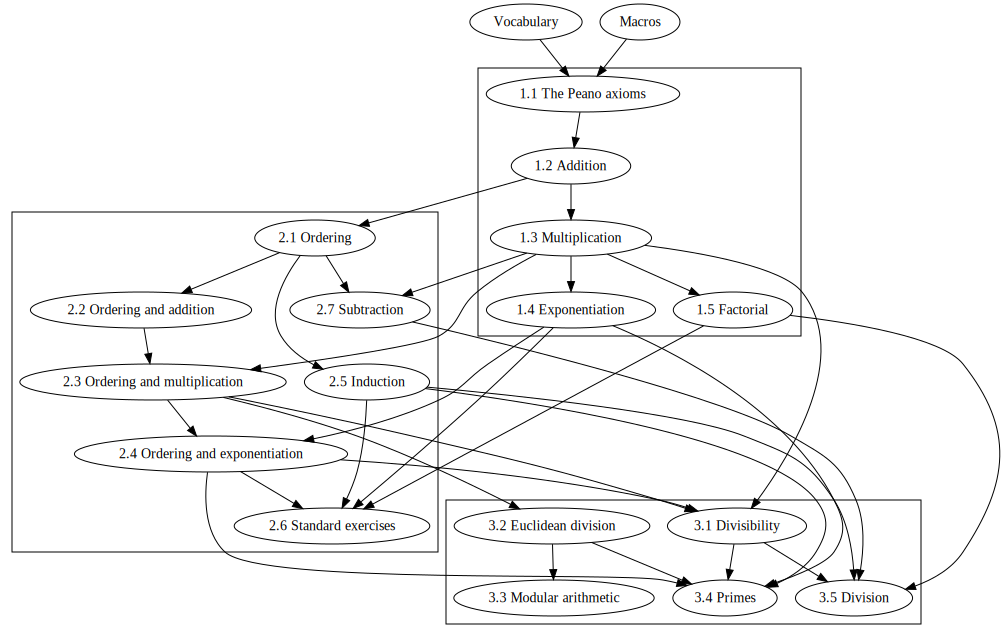
\includegraphics[width=0.9\linewidth]{./dependency-graph/graph.png}}
    \caption*{Interdependencies of the chapters}
  \end{figure}


  \section*{Introduction}

  This is a library providing a foundation of mathematics based on a
  Kelley-Morse like class theory with urelements.
  It introduces common operations on classes like unions or intersections
  (\cref{chapter:classes}) together with detailed proofs of their algebraic
  properties (\cref{chapter:computation-laws-for-classes}), the symmetric
  difference of two classes (\cref{chapter:symmetric-difference}) and the
  notions of ordered pairs and Cartesian products
  (\cref{chapter:pairs-and-products}) as well as proofs of the algebraic
  properties of the latter (\cref{chapter:computation-laws-for-products}).
  Moreover, it provides common operations on maps (\cref{chapter:maps}), various
  properties of images and preimages (\cref{chapter:image-and-preimage}) and the
  notions of injectivity, surjectivity, bijectivity
  (\cref{chapter:injections-surjections-bijections}) and invertibility of maps
  (\cref{chapter:invertible-maps}).
  The library provides an axiom system characterizing sets (\cref{chapter:sets})
  and, furthermore, it covers the notions of binary relations
  (\cref{chapter:binary-relations}), fixed-points of subset preserving maps
  (\cref{chapter:fixed-points}), including and equinumerosity
  (\cref{chapter:equinumerosity}).

  As two famous results it includes the Knaster-Tarski fixed point theorem
  (\cref{FOUNDATIONS_12_8420450166112256}) and the Cantor-Schröder-Bernstein
  theorem (\cref{FOUNDATIONS_13_1913663275401216}).

  \paragraph*{Usage.}
  At the very beginning of each chapter you can find the name of its source
  file, e.g. \path{foundations/sections/01_classes.ftl.tex} for
  \cref{chapter:classes}. This filename can be used to import the chapter via
  \Naproche's \texttt{readtex} instruction to another ForTheL text, e.g.:
  \begin{center}
    \verb`[readtex \path{foundations/sections/01_classes.ftl.tex}]`
  \end{center}

  \paragraph*{Checking times.}
  The checking times for each of the chapters may vary from computer to
  computer, but on mid-range hardware they are likely to be similar to those
  given in table below:

  \begin{center}
    \begin{tabular}{c|c|c}

      & \multicolumn{2}{c}{\textbf{Checking time}}
      \\
      \textbf{Chapter}
      & \textbf{without dependencies}     & \textbf{with dependencies}
      \\ \hline
      \ref{chapter:classes}
      & 00:04 min                         & 00:04 min
      \\
      \ref{chapter:computation-laws-for-classes}
      & 00:12 min                         & 00:16 min
      \\
      \ref{chapter:symmetric-difference}
      & 00:32 min                         & 00:48 min
      \\
      \ref{chapter:pairs-and-products}
      & 00:08 min                         & 00:12 min
      \\
      \ref{chapter:computation-laws-for-products}
      & 01:36 min                         & 01:56 min
      \\
      \ref{chapter:maps}
      & 01:13 min                         & 01:25 min
      \\
      \ref{chapter:image-and-preimage}
      & 01:28 min                         & 02:53 min
      \\
      \ref{chapter:injections-surjections-bijections}
      & 00:38 min                         & 02:03 min
      \\
      \ref{chapter:invertible-maps}
      & 02:20 min                         & 04:23 min
      \\
      \ref{chapter:sets}
      & 02:17 min                         & 06:40 min
      \\
      \ref{chapter:binary-relations}
      & 00:14 min                         & 06:54 min
      \\
      \ref{chapter:fixed-points}
      & 00:33 min                         & 07:13 min
      \\
      \ref{chapter:equinumerosity}
      & 01:48 min                         & 09:01 min
    \end{tabular}
  \end{center}


  \subfile{sections/01_classes.ftl.tex}
  \subfile{sections/02_computation-laws-for-classes.ftl.tex}
  \subfile{sections/03_symmetric-difference.ftl.tex}
  \subfile{sections/04_pairs-and-products.ftl.tex}
  \subfile{sections/05_computation-laws-for-products.ftl.tex}
  \subfile{sections/06_maps.ftl.tex}
  \subfile{sections/07_image-and-preimage.ftl.tex}
  \subfile{sections/08_injections-surjections-bijections.ftl.tex}
  \subfile{sections/09_invertible-maps.ftl.tex}
  \subfile{sections/10_sets.ftl.tex}
  \subfile{sections/11_binary-relations.ftl.tex}
  \subfile{sections/12_fixed-points.ftl.tex}
  \subfile{sections/13_equinumerosity.ftl.tex}
\end{document}

\usepackage{amssymb}

\newcommand{\Nat}{\mathbb{N}}
\newcommand{\Prime}{\mathbb{P}}
\renewcommand{\succ}{\textrm{succ}}
\newcommand{\pred}{\textrm{pred}}
\newcommand{\add}{\textrm{add}}
\newcommand{\mul}{\textrm{mul}}
\renewcommand{\exp}{\textrm{exp}}
\newcommand{\fac}{\textrm{fac}}
\renewcommand{\div}{\mathop{\textrm{div}}}
\renewcommand{\mod}{\mathop{\textrm{mod}}}

\begin{document}
  \begin{imports}
    \begin{forthel}
      %[prove off][check off]
      [read \path{libraries/source/arithmetics/natural-numbers.ftl.tex}]
      %[prove on][check on]
    \end{forthel}
  \end{imports}


  \section*{The Standard Ordering of the Natural Numbers}

  \subsection*{Definitions and Immediate Consequences}

  \begin{forthel}
    \begin{definition}[id=ARITHMETIC_04_1926295512416256,printid]
      Let $n, m$ be natural numbers.
      $n < m$ iff there exists a nonzero natural number $k$ such that $m = n + k$.
    \end{definition}

    Let $n$ is less than $m$ stand for $n < m$.
    Let $n > m$ stand for $m < n$.
    Let $n$ is greater than $m$ stand for $n > m$.
    Let $n \nless m$ stand for $n$ is not less than $m$.
    Let $n \ngtr m$ stand for $n$ is not greater than $m$.
  \end{forthel}

  \begin{forthel}
    \begin{definition}[id=ARITHMETIC_04_3668680374222848,printid]
      Let $n$ be a natural number.
      $\Nat_{< n} = \{ k \in \Nat \mid k < n \}$.
    \end{definition}
  \end{forthel}

  \begin{forthel}
    \begin{definition}[id=ARITHMETIC_04_3670333934534656,printid]
      Let $n$ be a natural number.
      $\Nat_{> n} = \{ k \in \Nat \mid k > n \}$.
    \end{definition}
  \end{forthel}

  \begin{forthel}
    \begin{definition}[id=ARITHMETIC_04_7916616566177792,printid]
      Let $n$ be a natural number.
      $n$ is positive iff $n > 0$.
    \end{definition}
  \end{forthel}

  \begin{forthel}
    \begin{definition}[id=ARITHMETIC_04_4593841531256832,printid]
      Let $n, m$ be natural numbers.
      $n \leq m$ iff there exists a natural number $k$ such that $m = n + k$.
    \end{definition}

    Let $n$ is less than or equal to $m$ stand for $n \leq m$.
    Let $n \geq m$ stand for $m \leq n$.
    Let $n$ is greater than or equal to $m$ stand for $n \geq m$.
    Let $n \nleq m$ stand for $n$ is not less than or equal to $m$.
    Let $n \ngeq m$ stand for $n$ is not greater than or equal to $m$.
  \end{forthel}

  \begin{forthel}
    \begin{definition}[id=ARITHMETIC_04_72501526790144,printid]
      Let $n$ be a natural number.
      $\Nat_{\leq n} = \{ k \in \Nat \mid k \leq n \}$.
    \end{definition}
  \end{forthel}

  \begin{forthel}
    \begin{definition}[id=ARITHMETIC_04_1706933421604864,printid]
      Let $n$ be a natural number.
      $\Nat_{\geq n} = \{ k \in \Nat \mid k \geq n \}$.
    \end{definition}
  \end{forthel}

  \begin{forthel}
    \begin{proposition}[id=ARITHMETIC_04_5385415374667776,printid]
      Let $n, m$ be natural numbers.
      $n \leq m$ iff $n < m$ or $n = m$.
    \end{proposition}
    \begin{proof}
      Case $n \leq m$.
        Take a natural number $k$ such that $m = n + k$.
        If $k = 0$ then $n = m$. If $k \neq 0$ then $n < m$.
      End.

      Case $n < m$ or $n = m$.
        If $n < m$ then there is a positive natural number $k$ such that $m = n + k$.
        If $n = m$ then $m = n + 0$.
        Thus if $n < m$ then there is a natural number $k$ such that $m = n + k$.
      End.
    \end{proof}
  \end{forthel}

  \begin{forthel}
    \begin{definition}[id=ARITHMETIC_04_6232154608500736,printid]
      Let $n$ be a natural number.
      A predecessor of $n$ is a natural number that is less than $n$.
    \end{definition}
  \end{forthel}

  \begin{forthel}
    \begin{definition}[id=ARITHMETIC_04_8147686326796288,printid]
      Let $n$ be a natural number.
      A successor of $n$ is a natural number that is greater than $n$.
    \end{definition}
  \end{forthel}

  \begin{forthel}
    \begin{proposition}[id=ARITHMETIC_04_4826285599621120,printid]
      Let $n$ be a natural number.
      Then $n$ is positive iff $n$ is nonzero.
    \end{proposition}
    \begin{proof}
      Case $n$ is positive.
        Take a positive natural number $k$ such that $n = 0 + k = k$.
        Then we have $n \neq 0$.
      End.

      Case $n$ is nonzero.
        Take a natural number $k$ such that $n = k + 1$.
        Then $n = 0 + (k + 1)$.
        $k + 1$ is positive.
        Hence $0 < n$.
      End.
    \end{proof}
  \end{forthel}


  \subsection*{Basic Properties}

  \begin{forthel}
    \begin{proposition}[id=ARITHMETIC_04_1037693395927040,printid]
      Let $n$ be a natural number.
      Then \[ n \nless n. \]
    \end{proposition}
    \begin{proof}
      Assume the contrary.
      Then we can take a positive natural number $k$ such that $n = n + k$.
      Then we have $0 = k$.
      Contradiction.
    \end{proof}
  \end{forthel}

  \begin{forthel}
    \begin{proposition}[id=ARITHMETIC_04_8266284905005056,printid]
      Let $n, m$ be natural numbers.
      Then \[ n < m \implies n \neq m. \]
    \end{proposition}
    \begin{proof}
      Assume $n < m$.
      Take a positive natural number $k$ such that $m = n + k$.
      If $n = m$ then $k = 0$.
      Hence $n \neq m$.
    \end{proof}
  \end{forthel}

  \begin{forthel}
    \begin{proposition}[id=ARITHMETIC_04_4190604718243840,printid]
      Let $n, m$ be natural numbers.
      If $n \leq m$ and $m \leq n$ then $n = m$.
    \end{proposition}
    \begin{proof}
      Assume $n \leq m$ and $m \leq n$.
      Take natural numbers $k, l$ such that $m = n + k$ and $n = m + l$.
      Then $m
        = n + k
        = (m + l) + k
        = m + (l + k)$.
      Hence $l + k = 0$.
      Thus $l = 0 = k$.
      Indeed if $l \neq 0$ or $k \neq 0$ then $l + k$ is the direct successor of
      some natural number.
      Therefore $m = n$.
    \end{proof}
  \end{forthel}

  \begin{forthel}
    \begin{proposition}[id=ARITHMETIC_04_6413905244979200,printid]
      Let $n, m, k$ be natural numbers.
      If $n < m < k$ then $n < k$.
    \end{proposition}
    \begin{proof}
      Assume $n < m < k$.
      Take a positive natural number $a$ such that $m = n + a$.
      Take a positive natural number $b$ such that $k = m + b$.
      Then $k
        = m + b
        = (n + a) + b
        = n + (a + b)$.
      $a + b$ is positive.
      Hence $n < k$.
    \end{proof}
  \end{forthel}

  \begin{forthel}
    \begin{proposition}[id=ARITHMETIC_04_5480385953660928,printid]
      Let $n, m, k$ be natural numbers.
      If $n \leq m \leq k$ then $n \leq k$.
    \end{proposition}
    \begin{proof}
      Assume $n \leq m \leq k$.
      Case $n = m = k$. Obvious.
      Case $n = m < k$. Obvious.
      Case $n < m = k$. Obvious.
      Case $n < m < k$. Obvious.
    \end{proof}
  \end{forthel}

  \begin{forthel}
    \begin{proposition}[id=ARITHMETIC_04_5098403656630272,printid]
      Let $n, m, k$ be natural numbers.
      If $n \leq m < k$ then $n < k$.
    \end{proposition}
    \begin{proof}
      Assume $n \leq m < k$.
      If $n = m$ then $n < k$.
      If $n < m$ then $n < k$.
    \end{proof}
  \end{forthel}

  \begin{forthel}
    \begin{proposition}[id=ARITHMETIC_04_4809599527944192,printid]
      Let $n, m, k$ be natural numbers.
      If $n < m \leq k$ then $n < k$.
    \end{proposition}
    \begin{proof}
      Assume $n < m \leq k$.
      If $m = k$ then $n < k$.
      If $m < k$ then $n < k$.
    \end{proof}
  \end{forthel}

  \begin{forthel}
    \begin{proposition}[id=ARITHMETIC_04_8584998051381248,printid]
      Let $n, m$ be natural numbers.
      If $n < m$ then $n + 1 \leq m$.
    \end{proposition}
    \begin{proof}
      Assume $n < m$.
      Take a positive natural number $k$ such that $m = n + k$.

      Case $k = 1$.
        Then $m = n + 1$.
        Hence $n + 1 \leq m$.
      End.

      Case $k \neq 1$.
        Then we can take a natural number $l$ such that $k = l + 1$.
        Then $m
          = n + (l + 1)
          = (n + l) + 1
          = (n + 1) + l$.
        $l$ is positive.
        Thus $n + 1 < m$.
      End.
    \end{proof}
  \end{forthel}

  \begin{forthel}
    \begin{proposition}[id=ARITHMETIC_04_8201937860165632,printid]
      Let $n, m$ be natural numbers.
      Then $n < m$ or $n = m$ or $n > m$.
    \end{proposition}
    \begin{proof}
      Define $\Phi = \{ m' \in \Nat \mid n < m'$ or $n = m'$ or $n > m' \}$.

      (1) $\Phi$ contains $0$.

      (2) For all $m' \in \Phi$ we have $m' + 1 \in \Phi$. \\
      Proof.
        Let $m' \in \Phi$.

        Case $n < m'$. Obvious.

        Case $n = m'$. Obvious.

        Case $n > m'$.
          Take a positive natural number $k$ such that $n = m' + k$.

          Case $k = 1$. Obvious.

          Case$k \neq 1$.
            Take a natural number $l$ such that $n = (m' + 1) + l$.
            Hence $n > m' + 1$.
            Indeed $l$ is positive.
          End.
        Qed.
      Qed.

      Thus every natural number is contained in $\Phi$ (by \printref{ARITHMETIC_01_4764664342773760}).
      Therefore $n < m$ or $n = m$ or $n > m$.
    \end{proof}
  \end{forthel}

  \begin{forthel}
    \begin{proposition}[id=ARITHMETIC_04_6991525988794368,printid]
      Let $n, m$ be natural numbers.
      Then $n \nless m$ iff $n \geq m$.
    \end{proposition}
    \begin{proof}
      Case $n \nless m$.
        Then $n = m$ or $n > m$.
        Hence $n \geq m$.
      End.

      Case $n \geq m$.
        Assume $n < m$.
        Then $n \leq m$.
        Hence $n = m$.
        Contradiction.
      End.
    \end{proof}
  \end{forthel}


  \subsection*{Ordering and Successors}

  \begin{forthel}
    \begin{proposition}[id=ARITHMETIC_04_7006203091615744,printid]
      Let $n, m$ be natural numbers.
      If $n < m \leq n + 1$ then $m = n + 1$.
    \end{proposition}
    \begin{proof}
      Assume $n < m \leq n + 1$.
      Take a positive natural number $k$ such that $m = n + k$.
      Take a natural number $l$ such that $n + 1 = m + l$.
      Then $n + 1
        = m + l
        = (n + k) + l
        = n + (k + l)$.
      Hence $k + l = 1$.

      We have $l = 0$. \\
      Proof.
        Assume the contrary.
        Then $k,l > 0$.

        Case $k,l = 1$.
          Then $k + l
            = 2
            \neq 1$.
          Contradiction.
        End.

        Case $k = 1 and l \neq 1$.
          Then $l > 1$.
          Hence $k + l
            > 1 + l
            > 1$.
          Contradiction.
        End.

        Case $k \neq 1 and l = 1$.
          Then $k > 1$.
          Hence $k + l
            > k + 1
            > 1$.
          Contradiction.
        End.

        Case $k, l \neq 1$.
          Take natural numbers $a, b$ such that $k = a + 1$ and $l = b + 1$.
          Indeed $k, l \neq 0$.
          Hence $k = a + 1$ and $l = b + 1$.
          Thus $k, l > 1$. Indeed $a, b$ are positive.
        End.
      Qed.

      Then we have $n + 1
        = m + l
        = m + 0
        = m$.
    \end{proof}
  \end{forthel}

  \begin{forthel}
    \begin{proposition}[id=ARITHMETIC_04_8792330561650688,printid]
      Let $n, m$ be natural numbers.
      If $n \leq m < n + 1$ then $n = m$.
    \end{proposition}
    \begin{proof}
      Assume $n \leq m < n + 1$.

      Case $n = m$. Obvious.

      Case $n < m$.
        Then $n < m \leq n + 1$.
        Hence $n = m$.
      End.
    \end{proof}
  \end{forthel}

  \begin{forthel}
    \begin{corollary}[id=ARITHMETIC_04_1802826644717568,printid]
      Let $n$ be a natural number.
      There is no natural number $m$ such that $n < m < n + 1$.
    \end{corollary}
    \begin{proof}
      Assume the contrary.
      Take a natural number $m$ such that $n < m < n + 1$.
      Then $n < m \leq n + 1$ and $n \leq m < n + 1$.
      Hence $m = n + 1$ and $m = n$.
      Hence $n = n + 1$.
      Contradiction.
    \end{proof}
  \end{forthel}

  \begin{forthel}
    \begin{proposition}[id=ARITHMETIC_04_990407185924096,printid]
      Let $n$ be a natural number.
      Then $n + 1 \geq 1$.
    \end{proposition}
    \begin{proof}
      Case $n = 0$. Obvious.

      Case $n \neq 0$.
        Then $n > 0$.
        Hence $n + 1 > 0 + 1 = 1$.
      End.
    \end{proof}
  \end{forthel}


  \subsection*{Ordering and Addition}

  \begin{forthel}
    \begin{proposition}[id=ARITHMETIC_04_7354062662008832,printid]
      Let $n, m, k$ be natural numbers.
      Then $n < m$ iff $n + k < m + k$.
    \end{proposition}
    \begin{proof}
      Case $n < m$.
        Take a positive natural number $l$ such that $m = n + l$.
        Then $m + k
          = (n + l) + k
          = (n + k) + l$.
        Hence $n + k < m + k$.
      End.

      Case $n + k < m + k$.
        Take a positive natural number $l$ such that $m + k = (n + k) + l$.
        $(n + k) + l
          = n + (k + l)
          = n + (l + k)
          = (n + l) + k$.
        Hence $m + k = (n + l) + k$.
        Thus $m = n + l$ (by \printref{ARITHMETIC_03_3137702874578944}).
        Therefore $n < m$.
      End.
    \end{proof}
  \end{forthel}

  \begin{forthel}
    \begin{corollary}[id=ARITHMETIC_04_1901366129721344,printid]
      Let $n, m, k$ be natural numbers.
      Then $n < m$ iff $k + n < k + m$.
    \end{corollary}
    \begin{proof}
      We have $k + n = n + k$ and $k + m = m + k$.
      Hence $k + n < k + m$ iff $n + k < m + k$.
    \end{proof}
  \end{forthel}

  \begin{forthel}
    \begin{corollary}[id=ARITHMETIC_04_4203390999461888,printid]
      Let $n, m, k$ be natural numbers.
      Then $n \leq m$ iff $k + n \leq k + m$.
    \end{corollary}
  \end{forthel}

  \begin{forthel}
    \begin{corollary}[id=ARITHMETIC_04_5512590832697344,printid]
      Let $n, m, k$ be natural numbers.
      Then $n \leq m$ iff $n + k \leq m + k$.
    \end{corollary}
  \end{forthel}


  \subsection*{Induction Revisited}

  \begin{forthel}
    \begin{proposition}[id=ARITHMETIC_04_272317502455808,printid]
      Let $A$ be a nonempty subclass of $\Nat$.
      Then there exists a $m \in A$ such that $m \leq n$ for all $n \in A$.
    \end{proposition}
    \begin{proof}
      Assume the contrary.

      Let us show that for each $n \in A$ there exists a $m \in A$ such that $m < n$.
        Let $n \in A$.
        Assume that there exists no $m \in A$ such that $m < n$.
        Then $n \leq m$ for all $m \in A$.
        Contradiction.
      End.

      (a) Define $\Phi = \{ n \in \Nat \mid n$ is less than any element of $A \}$.

      (1) $\Phi$ contains $0$. \\
      Proof.
        $0 \notin A$.
        Hence $0$ is less than every element of $A$.
        Thus $0 \in \Phi$.
      Qed.

      (2) For all $n \in \Phi$ we have $n + 1 \in \Phi$. \\
      Proof.
        Let $n \in \Phi$.
        Then $n$ is less than any element of $A$.
        Assume that $\Phi$ does not contain $n + 1$.
        Then we can take an $m \in A$ such that $n + 1 \nless m$ (by a).
        Then $n < m \leq n + 1$.
        Hence $m = n + 1$.
        Contradiction.
      Qed.

      Then $\Phi$ contains every natural number (by \printref{ARITHMETIC_01_4764664342773760}).
      Therefore every natural number is less than any element of $A$.
      Consequently $A$ has no elements.
      Contradiction.
    \end{proof}
  \end{forthel}

  \begin{forthel}
    \begin{theorem}[id=ARITHMETIC_04_3609801697263616,printid]
      Let $A$ be a class.
      Assume for all $n \in \Nat$ if $A$ contains all predecessors of $n$ then $A$ contains $n$.
      Then $A$ contains every natural number.
    \end{theorem}
    \begin{proof}
      Assume the contrary.
      Take a natural number $n$ that is not contained in $A$.
      Then $n$ is contained in $\Nat \setminus A$.
      Hence we can take a $m \in \Nat \setminus A$ such that $m \leq k$ for all $k \in \Nat \setminus A$.
      Then $\Nat \setminus A$ does not contain any predecessor of $m$.
      Therefore $A$ contains all predecessors of $m$.
      Consequently $A$ contains $m$.
      Contradiction.
    \end{proof}
  \end{forthel}

  \begin{forthel}
    \begin{theorem}[id=ARITHMETIC_04_4976599269113856,printid]
      Let $A$ be a class.
      Let $k$ be a natural number such that $k \in A$.
      Assume that for all $n \in \Nat_{\geq k}$ if $n \in A$ then $n + 1 \in A$.
      Then for all $n \in \Nat_{\geq k}$ we have $n \in A$.
    \end{theorem}
    \begin{proof}
      Define $\Phi = \{n \in \Nat \mid$ if $n \geq k$ then $n \in A \}$.

      (1) $\Phi$ contains $0$.
      Indeed if $0 \geq k$ then $0 = k \in A$.

      (2) For all $n \in \Phi$ we have $n + 1 \in \Phi$. \\
      Proof.
        Let $n \in \Phi$.

        Let us show that if $n + 1 \geq k$ then $n + 1 \in A$.
          Assume $n + 1 \geq k$.

          Case $n < k$.
            Then $n + 1 = k$.
            Hence $n + 1 \in A$.
          End.

          Case $n \geq k$.
            Then $n \in A$.
            Hence $n + 1 \in A$.
          End.
        End.

        Therefore $n + 1 \in \Phi$.
      Qed.

      Thus $\Phi$ contains every natural number (by \printref{ARITHMETIC_01_4764664342773760}).
      Consequently for all $n \in \Nat_{\geq k}$ we have $n \in A$.
    \end{proof}
  \end{forthel}
\end{document}
